\documentclass[12pt,spanish,a5paper,landscape]{article}
\usepackage[utf8]{inputenc}
\usepackage{babel}
\usepackage{listings}
\usepackage{mathpazo}
\usepackage{courier}
\usepackage{textcomp}
\usepackage[parfill]{parskip}
\usepackage{xcolor}
\usepackage[margin=1.5cm]{geometry}
\usepackage{enumitem}
\usepackage{microtype}

\newcommand{\onelinerule}{\rule[2.3ex]{0pt}{0pt}}
\newcommand{\twolinerule}{\rule[6.2ex]{0pt}{0pt}}
\newcommand{\respuesta}{\framebox[\textwidth]{\twolinerule}}
\newcommand{\nombre}{%
  \begin{tikzpicture}[xscale=.4,yscale=.7]
    \draw (0, 0) rectangle (22, 1);
  \end{tikzpicture}%
}
%\newcommand{\rol}   {\framebox[0.3\textwidth]{\onelinerule}}
\newcommand{\rol}{%
  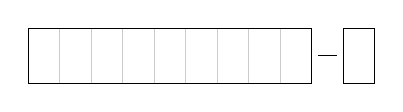
\begin{tikzpicture}[xscale=.4,yscale=.7]
    \draw[gray!40] ( 0, 0) grid      ( 9, 1);
    \draw          ( 0, 0) rectangle ( 9, 1);
    \draw          (10, 0) rectangle (11, 1);
    \draw (9 + .2, .5) -- (10 - .2, .5);
  \end{tikzpicture}%
}
\newcommand{\li}{\lstinline}
\providecommand{\pond}[1]{[{\small\textbf{#1\%}}]}

\lstdefinelanguage{py}{%
  classoffset=0,%
    morekeywords={%
      False,class,finally,is,return,None,continue,for,lambda,try,%
      True,def,from,nonlocal,while,and,del,global,not,with,print,%
      as,elif,if,or,yield,assert,else,import,pass,break,except,in,raise},%
    keywordstyle=\color{black!80}\bfseries,%
  classoffset=1,
    morekeywords={int,float,str,abs,len,raw_input,exit,range,min,max,%
      set,dict,tuple,list,bool,complex,round,sum,all,any,zip,map,filter,%
      sorted,reversed,dir,file,frozenset,open,%
      array,zeros,ones,arange,linspace,eye,diag,dot},
    keywordstyle=\color{black!50}\bfseries,%
  classoffset=0,%
  sensitive=true,%
  morecomment=[l]\#,%
  morestring=[b]',%
  morestring=[b]",%
  stringstyle=\em,%
}

\lstdefinelanguage{testcase}{%
  moredelim=[is][\bfseries]{`}{`},%
  backgroundcolor=\color{gray!20},%
}

\lstdefinelanguage{file}{%
  frame=single,%
}

\lstset{language=py}
\lstset{basicstyle=\ttfamily}
\lstset{columns=fixed}
\lstset{upquote=true}
\lstset{showstringspaces=false}
\lstset{rangeprefix=\#\ }
\lstset{includerangemarker=false}

\newlist{certamen}{enumerate}{1}
\setlist[certamen]{%
  label=\arabic*.,
  font=\LARGE\bfseries,%
  labelindent=-.5in,%
  leftmargin=0pt,%
  labelsep=1em%
}


\lstset{language=testcase}
\lstset{frame=single}

\begin{document}
  \pagestyle{empty}
  \thispagestyle{empty}

  \part*{Control 5, lunes 1--2}
  \newpage

  \begin{minipage}[t]{0.45\textwidth}
    El archivo \li!diccionario.txt!
    contiene las definiciones de varias palabras
    en el formato mostrado a la derecha.
    \\[2ex]
    Cada línea del archivo tiene una palabra y su definición,
    separados por dos puntos.
    Además, junto a cada palabra,
    se indica si ésta es un sustantivo \li!(s)!
    o un verbo \li!(v)!.
  \end{minipage}
  \hfill
  \begin{minipage}[t]{0.45\textwidth}
    \hfil\verb!diccionario.txt!\hfil
    \small
    \lstinputlisting[language=file]{diccionario.txt}
  \end{minipage}

  Escriba un programa que pregunte al usuario una palabra,
  y entregue como salida su definición y su tipo de palabra.
  Si la palabra no está en el diccionario,
  el programa debe mostrar el mensaje
  \texttt{La palabra no esta en el diccionario}.

  Use los siguientes ejemplos como referencia.

  \begin{minipage}[t]{0.6\textwidth}
    \lstinputlisting[linerange=CASO\ 1-FIN\ CASO\ 1]{lunes-1-2.py}
  \end{minipage}

  \begin{minipage}[t]{0.6\textwidth}
    \lstinputlisting[linerange=CASO\ 2-FIN\ CASO\ 2]{lunes-1-2.py}
  \end{minipage}

  \newpage

  \part*{Control 5, lunes 3--4}
  \newpage

  \newpage

  \part*{Control 5, martes 1--2}
  \newpage

  \newpage

  \part*{Control 5, martes 3--4}
  \newpage

  \begin{minipage}[t]{0.48\textwidth}
    Rosalinda Sansana mantiene su horario de este semestre
    en un archivo llamado \li!horario.txt!,
    siguiendo el formato mostrado a la derecha.
    \\[2ex]
    En cada línea del archivo aparece el nombre de un ramo
    seguido de dos puntos.
    A continuación,
    aparecen todas las clases de ese ramo en la semana,
    separados por comas.
    Los nombres de los días están abreviados
    por sus dos primeras letras.
  \end{minipage}
  \hfill
  \begin{minipage}[t]{0.42\textwidth}
    \hfil\verb!horario.txt!\hfil
    \lstinputlisting[language=file]{horario.txt}
  \end{minipage}

  Escriba un programa que le pregunte a Rosalinda
  cuál es el día de hoy,
  y le diga cuáles son las clases que debe asistir
  y en qué bloques.

  \begin{minipage}[t]{0.6\textwidth}
    \lstinputlisting[linerange=CASO-FIN\ CASO]{martes-3-4.py}
  \end{minipage}

\end{document}

